\documentclass{standalone}
\usepackage{tikz}
\usetikzlibrary{lindenmayersystems}
\usepackage{pgfplots}

\begin{document}
%\tikz \draw[] (0,0) [koch=7];
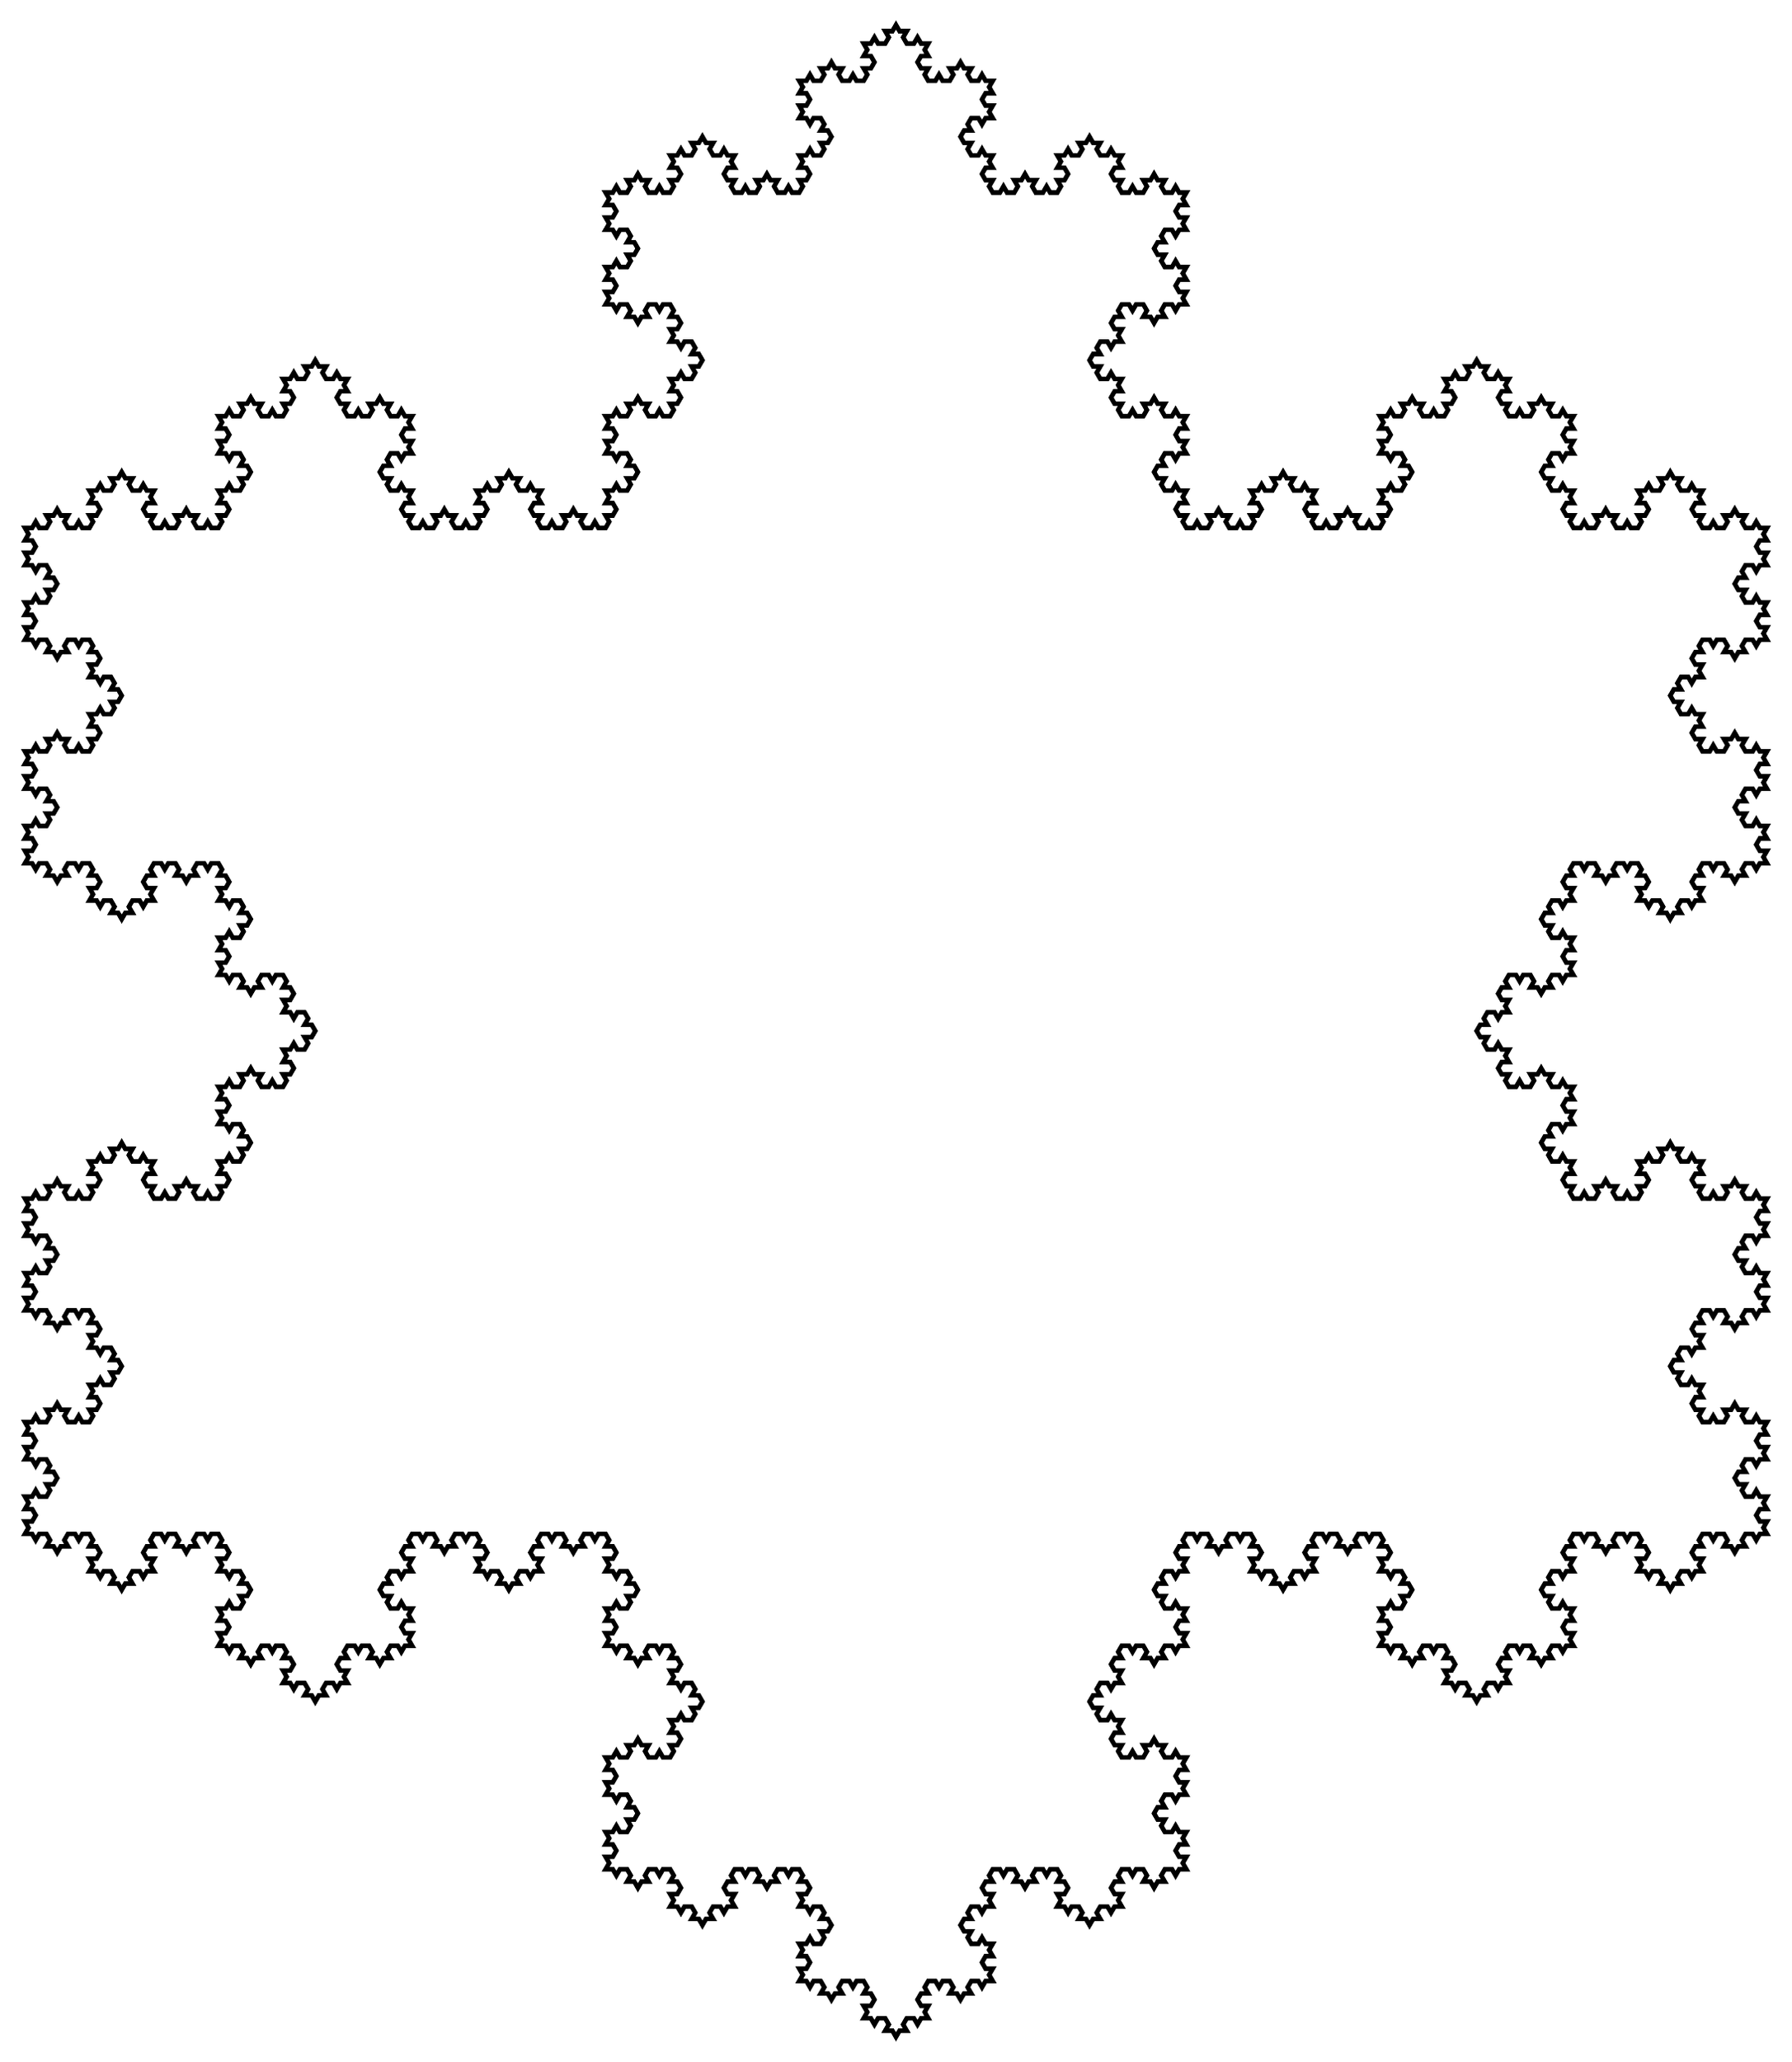
\begin{tikzpicture}
\pgfdeclarelindenmayersystem{Koch curve}{
  \rule{F -> F-F++F-F}
}


\begin{scope}[xshift = 0cm]
\draw[l-system={Koch curve, step=0.11111111111cm, angle=60, axiom=F++F++F, order=5}, line width=2pt]
lindenmayer system -- cycle;
\end{scope}
\end{tikzpicture}
\end{document}